\documentclass[preview]{standalone}

\usepackage{amsmath}
\usepackage{amssymb}
\usepackage{stellar}
\usepackage{bettelini}

\hypersetup{
    colorlinks=true,
    linkcolor=black,
    urlcolor=blue,
    pdftitle={Biologia},
    pdfpagemode=FullScreen,
}

\begin{document}

\title{Biologia}
\id{biologia-sistemi-viventi}
\genpage

\begin{snippetdefinition}{atp-definizione}{ATP}
    ATP è un composto organico che provvede energia alle cellule per le loro funzioni.
\end{snippetdefinition}

\plain{I seguenti processi sono eseguiti da tutti gli organismi viventi.}

\plain{<b>→ Nutrizione:</b>}

\begin{snippet}{nutrizione-expl1}
Tutti gli organismi viventi si nutrono con del \quotes{cibo}, ossia materia.
In generale, gli esseri viventi necessitano di \(C\), \(O\), \(H\), \(N\), \(S\) e \(P\).
L'unico nutrimento della pianta è CO\({}_2\) (materia inorganica), mentre
i nutrimenti degli animali sono materia organica.
\end{snippet}

\begin{snippetdefinition}{autotrofo-definizione}{Autotrofo}
    Un organismo \textit{autotrofo} può svolgere la propria funzione di nutrizione,
    elaborando alimenti inorganici mediante assunzione d'energia dal mondo inorganico.
\end{snippetdefinition}

\begin{snippetdefinition}{eterotrofo-definizione}{Eterotrofo}
    Un organismo \textit{eterotrofo}
    si nutre di sostanze organiche prodotte dagli organismi autotrofi.
\end{snippetdefinition}

\plain{<b>→ Respirazione:</b>}

\begin{snippet}{respirazione-expl1}
Tutti gli organismi viventi respirano
\[
    C_6H_{12}O_6 + O_2 \rightarrow CO_2 + H_2O
\]
In assenza di ossigeno (si usa la materia organica per produrre energia), e alcuni organismi \textit{fermentano}.
Nel caso degli umani i muscoli respirano, se non c'è \(O\) fermentano e producono acido lattico
che deve successivamente essere smaltito.

Le piante respirano mediante la fotosintesi
\[
    CO_2 + H_2O \rightarrow C_6H_{12}O_6 + O_2
\]
\end{snippet}

\plain{<b>→ Si riproduce e ha un ciclo vitale;</b>}
\plain{<b>→ Evolve;</b>}
\plain{<b>→ È sensibile (sa rispondere all'ambiente);</b>}
\plain{<b>→ Mantiene stabili le sue condizioni interne.</b>}

\begin{snippetdefinition}{biotico-definizione}{Biotico}
    Con \textit{biotico} si intende tutto ciò che è vivente o era vivente.
\end{snippetdefinition}
% foglia morta, elefante

\begin{snippetdefinition}{abiotico-definizione}{Abiotico}
    Con \textit{abiotico} si intende tutto ciò che non è vivente e non lo è mai stato.
\end{snippetdefinition}
% roccia

\begin{snippetdefinition}{detrito-definizione}{Detrito}
    Con \textit{detrito} si intende il resto di ogni organismo vivente che è morto.
\end{snippetdefinition}
% % foglia morta

\plain{Il sistema vivente presenta le medesima ma caratteristiche del sistema non-vivente,
ma possiede anche le seguenti componenti.}

\begin{snippetdefinition}{componente-definizione}{Componente}
    Insieme di materia, concreta e tangibile.
\end{snippetdefinition}

\begin{snippetexample}{componenti-esempio}{Componenti}
    Acqua, suolo, sali minerali, ossigeno.
\end{snippetexample}

\begin{snippetdefinition}{fattore-definizione}{Fattore}
    Derive dalla presenza di componenti, produce un determinato effetto o risultato e si può misurare.
\end{snippetdefinition}

\begin{snippetexample}{fattore-esempio}{Fattore}
    \begin{itemize}
        \item Decomposizione (fattore biotico).
        \item Predazione, catena alimentare (fattore biotico).
        \item Vento (fattore abiotico).
        \item Luce solare (fattore abiotico).
        \item Luce della lucciola (fattore biotico).
    \end{itemize}
\end{snippetexample}

\plain{Un fattore rappresenta tutto ciò che si può misurare e che non è una componente.}

\plain{Ogni essere vivente possiede <b>autopoiesi</b>, <b>dissipazione</b> e <b>cognizione</b>.}

\section{Autopoiesi}

\begin{snippetdefinition}{autopoiesi-definizione}{Autopoiesi}
    La capacità di ripararsi, modificarsi e riprodursi da solo, internamente ed in maniera autonoma.
\end{snippetdefinition}

\plain{I sistemi viventi sono organizzativamente chiusi, per cui hanno un confine.}

\plain{<b>Sistema autopoietico (ciclo):</b>}

\begin{snippet}{sis-autop-ciclo-illustration}
    \begin{center}
    \begin{figure}[ht]
        \centering
        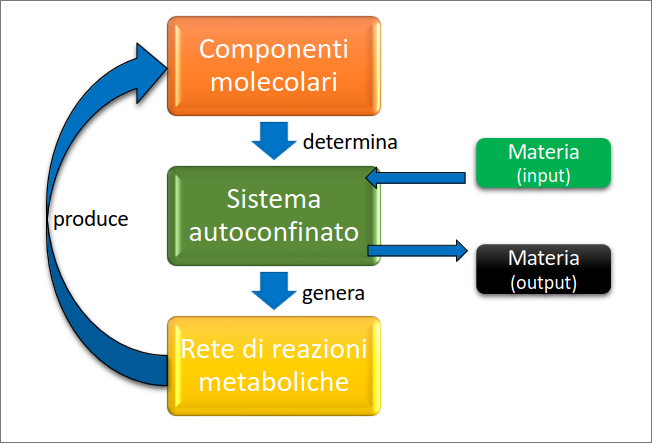
\includegraphics[width=0.65\textwidth]{./resources/sis_autop_ciclo.png}
    \end{figure}
    \end{center}
\end{snippet}

\plain{<b>Sistema autopoietico (cellula):</b>}

\begin{snippet}{sis-autop-cellula-illustration}
    \begin{center}
    \begin{figure}[ht]
        \centering
        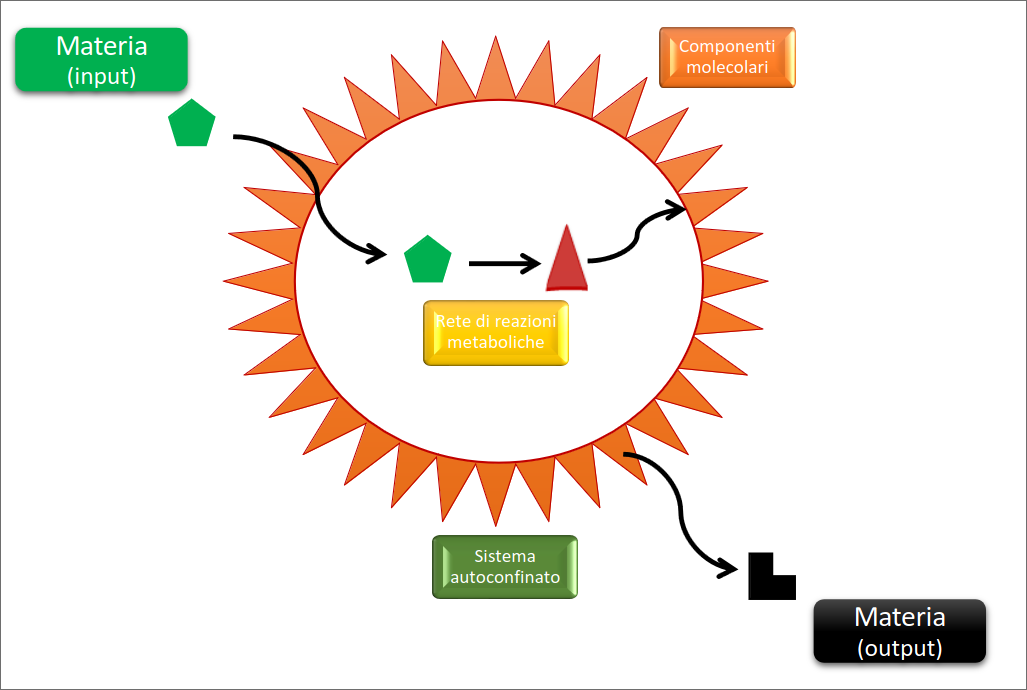
\includegraphics[width=0.65\textwidth]{./resources/sis_autop_cellula.png}
    \end{figure}
    \end{center}
\end{snippet}

\section{Dissipazione}

\begin{snippetdefinition}{dissipazione-definizione}{Dissipazione}
    La necessità di consumare energia, materia ed informazioni dall'esterno.
\end{snippetdefinition}

\plain{I sistemi viventi sono metabolicamente aperti, per cui hanno degli scambi con l'esterno
e rinnovano il proprio materiale.}

\section{Cognizione}

\begin{snippetdefinition}{cognizione-definizione}{Cognizione}
    L'attiva conoscenza dell'ambiente, esterno ed interno, da parte del sistema.
\end{snippetdefinition}

\end{document}